\section{Informatica}
\subsection{Conversione binario esadecimale}
La conversione numerica si ottiene raggruppando i bit del numero binario in gruppi da quattro a partire dal punto e in entrambe le direzioni, sostituendo poi ogni gruppo di 4 bit con l'equivalente cifra del sistema esadecimale.
\begin{multicols}{2}
\begin{itemize}
    \item 0000 = 0
    \item 0001 = 1
    \item 0010 = 2
    \item 0011 = 3
    \item 0100 = 4
    \item 0101 = 5
    \item 0110 = 6
    \item 0111 = 7
    \item 1000 = 8
    \item 1001 = 9
    \item 1010 = A
    \item 1011 = B
    \item 1100 = C
    \item 1101 = D
    \item 1110 = E
    \item 1111 = F
\end{itemize}
\end{multicols}
\subsection{Tipologia reti}
Le reti di telecomunicazione sono costituite da un insieme di nodi e rami che consentono la trasmissione di informazioni tra i vari nodi. Le reti possono essere classificate in base a diversi criteri:
\begin{itemize}
    \item \textbf{Estensione geografica:}
    \begin{itemize}
        \item \textbf{PAN} (Personal Area Network): copre pochi metri, ad esempio collegamento tra dispositivi personali (Bluetooth).
        \item \textbf{LAN} (Local Area Network): copre un edificio o un campus, tipicamente reti aziendali o domestiche.
        \item \textbf{MAN} (Metropolitan Area Network): copre una città o un'area metropolitana.
        \item \textbf{WAN} (Wide Area Network): copre aree geografiche molto estese, anche nazioni o continenti (es. Internet).
    \end{itemize}
    \item \textbf{Topologia:}
    \begin{itemize}
        \item \textbf{Bus}: tutti i nodi sono collegati a un unico canale di comunicazione.
        \item \textbf{Stella}: tutti i nodi sono collegati a un nodo centrale.
        \item \textbf{Anello}: i nodi sono collegati in modo circolare.
        \item \textbf{Maglia (mesh)}: ogni nodo è collegato a più nodi, anche direttamente.
        \item \textbf{Albero}: struttura gerarchica a livelli.
        \item \textbf{Catena (chain)}: i nodi sono collegati in sequenza lineare.
        \item \textbf{Full mesh}: ogni nodo è collegato a tutti gli altri nodi.
    \end{itemize}

\end{itemize}
\subsubsection{Nodi e rami}
I nodi e i rami(link) sono gli elementi che costituiscono una rete. I nodi sono i punti di intersezione tra i rami e possono essere di diversi tipi:
\begin{itemize}
    \item Host: un nodo che genera o consuma informazioni
    \item Router: un nodo che instrada le informazioni tra i vari host
    \item Switch: un nodo che instrada le informazioni tra i vari host, ma a livello di collegamento
    \item Bridge: un nodo che collega due reti locali
    \item Gateway: un nodo che collega due reti diverse
\end{itemize}
Il ramo è il sistema trasmissivo che consente il trasporto delle
unità informative da nodo a nodo secondo tre possibili modalità di trasmissione:
\begin{itemize}
    \item simplex(unidirezionale): un solo verso di trasmissione, esempio: radio
    \item half-duplex(bidirezionale alternato): due direzioni di trasmissione, ma non contemporaneamente, esempio: walkie-talkie
    \item full-duplex(bidirezionale contemporanea): due direzioni di trasmissione contemporaneamente, esempio: telefono
    \item broadcast: un nodo invia informazioni a tutti gli altri nodi della rete, esempio: radio
\end{itemize}

\paragraph{Modalità di invio dati}
\begin{itemize}
    \item broadcast: un nodo invia informazioni a tutti i nodi della rete, esempio: radio
    \item multicast: un nodo invia informazioni a un gruppo di nodi della rete, esempio: videoconferenza
    \item unicast: un nodo invia informazioni a un solo nodo della rete, esempio: email
    \item point-to-point: un nodo invia informazioni a un altro nodo della rete, esempio: telefono
\end{itemize}

\subsubsection{Reti di accesso e reti di trasporto}
Se mando una richiesta sul web tramite il mio router di casa, collegandomi alla rete tim(rete di accesso), da quel punto in poi tim si appoggerà ad un’altra rete per rispondere alla mia richiesta(rete di trasporto), quindi è possibile distinguere velocità differenti: 
\begin{itemize}
    \item velocità di accesso(relativa ai dati che viaggiano nella rete di accesso, tipicamente agli utenti semplici non viene garantita una velocità minima(da casa non abbiamo questa garanzia), nella rete di trasporto invece viene garantita(contratto SLA))
    \item velocità di trasporto(relativa ai dati che viaggiano nella rete di trasporto)
\end{itemize}

\subsection{Da analogico a digitale}
in base al tipo di comunicazione decido il modo con il quale mettere in comunicazione gli utenti, se sono tanti o pochi, se sono distanti o vicini, se comunicano contemporaneamente oppure no.
quando l’informazione che voglio trasmettere la digitallizzo, passando da analogico a digitale, ho molti vantaggi:
campionando il segnale analogico posso ricorstruirlo in segnale digitale, in bit.
quando chiamo qualcuno avviene il campionamento dell’onda audio della voce, questo avviene tramite il filtro passa banda tra le frequenze 300hz e 3400 hz. le alte e le bassissime frequenze vengono tagliate. 8 bit per campione, 64bit per secondo, quindi 8 campioni al secondo. la trasmissione nel canale telefonico avviene con la trasmissione di pacchetti.


\newpage
\section{Matematica}
\subsection{Aritmetica a 2 - XOR}
\subsection{Distribuzione di Poisson}
\section{Fisica}
\subsection{Comunicazione radio, cablata e ottica}
la trasmissione di un segnale a distanza avviene attraverso le onde elettromagnetiche, che siano trasmesse tramite antenne e quindi che si propaghino nel vuoto oppure in un cavo di fibra ottica, che anchesso trasmette la luce, quindi l’onda em.
dopo aver trasformato l'informazione in bit(codifica) questa viene trasmessa in dei canali(radio, mezzi guidati). quella radio avviene nello spazio libero(attraverso l’aria o nel vuoto), mezzi guidati(cavi)
\begin{itemize}
    \item Mezzi guidati: cavi coassiali, cavi in fibra ottica, cavi in rame
    \item Mezzi non guidati: onde radio, microonde, infrarossi
    \item Mezzi ottici: fibra ottica
\end{itemize}
\paragraph{Pro e contro del canale radio}
\begin{itemize}    
    \item Pro: risparmio sul mezzo fisico(l’aria e il vuoto sono gratis), un segnale radio non ha confini, può arrivare all’infinito, teoricamente. a noi interessa che il segnale elettromagnetico arrivi dove voglio e che venga decodificato correttamente, e non a infinito. 
un antenna è un dispositivo che genera un campo magnetico(è un pezzo di ferro su cui scorre della corrente e che quindi genera un campo magnetico, fisica 2), aiuta la comunicazione radio. 
    \item Contro: è più difficile gestire la privacy e sicurezza perchè il canale(l’aria, il vuoto) è condiviso tra tutti gli utenti. il canale radio ha più rumore(dovuto ad effetti naturali, il calore ad esempio) rispetto al cavo. l’interferenza è invece dovuta ad altre comunicazioni e non ad effetti naturali, nel canale radio anche l’interferenza può essere maggiore. il fading è un problema del canale radio, ossia il segnale non viaggia correttament per via di ostacoli come le montagne. problema dell’effetto doppler. problema dei cammini multipli
\end{itemize}
il mezzo radio è passabanda, in base alla frequenza con la quale l'onda viene trasmessa quest'ultima si comporta in modo differente. ad esempio a bassa frequenza si sfrutta il fenomeno del waving per il quale l'onda riflette sulla ionosfera e quindi si possono raggiungere distanze più elevate e per esempio attraversare l'oceano.
quando trasmetto via radio in base alla potenza con cui trasmetto regolo la frequenza con cui invio il segnale. maggiore potenza significa frequenza più alta. frequenza più alta vuol dire anche maggiore velocità di trasmissione ma copertura minore.
\paragraph{Canale radio e ostacoli fisici}
\begin{itemize}
    \item los(line of sight): il segnale radio non ha ostacoli, trasmissione diretta
    \item nlos(non line of sight): il segnale radio ha ostacoli, trasmissione non diretta
\end{itemize}
\paragraph{Mezzi guidati}
Esistono i mezzi guidati(cavi) come il doppino, il cavo coassiale e la fibra ottica.
il doppino ha al suo interno 2 fili, la corrente per scorrere ha bisogno di un circuito chiuso. infatti questo circuito chiuso si ottiene tramite due fili all’interno del cavo(doppino).
quindi si usa un doppino per trasmettere e un doppino per ricevere, quindi 4 fili in totale, cioè due circuiti chiusi. ricordare che i doppini possono essere di diversi tipi, viene principalmente usato il tipo UTP(unshielded twisted pair), coppia di conduttori intrecciati, non schermato(uno schermo serve ad evitare problemi con le correnti parassite, dovute ad altri fenomeni, non riguardano questo corso). quello schermato costa di più
il cavo coassiale ha 8 fili.
la fibra ottica trasmette onde em, non corrente (la corrente è un flusso di cariche elettriche e non è un'onda em), la banda di trasmissione è molto alta, $10^{14}$Hz.
I cavi in cui scorre corrente vengono tipicamente intrecciati per annullare gli effetti dei campi magnetici indotti in maniera vicendevole, così da non avere disturbo sul passaggio della corrente e quindi dell'informazione.
\begin{figure}[h!]
    \centering
    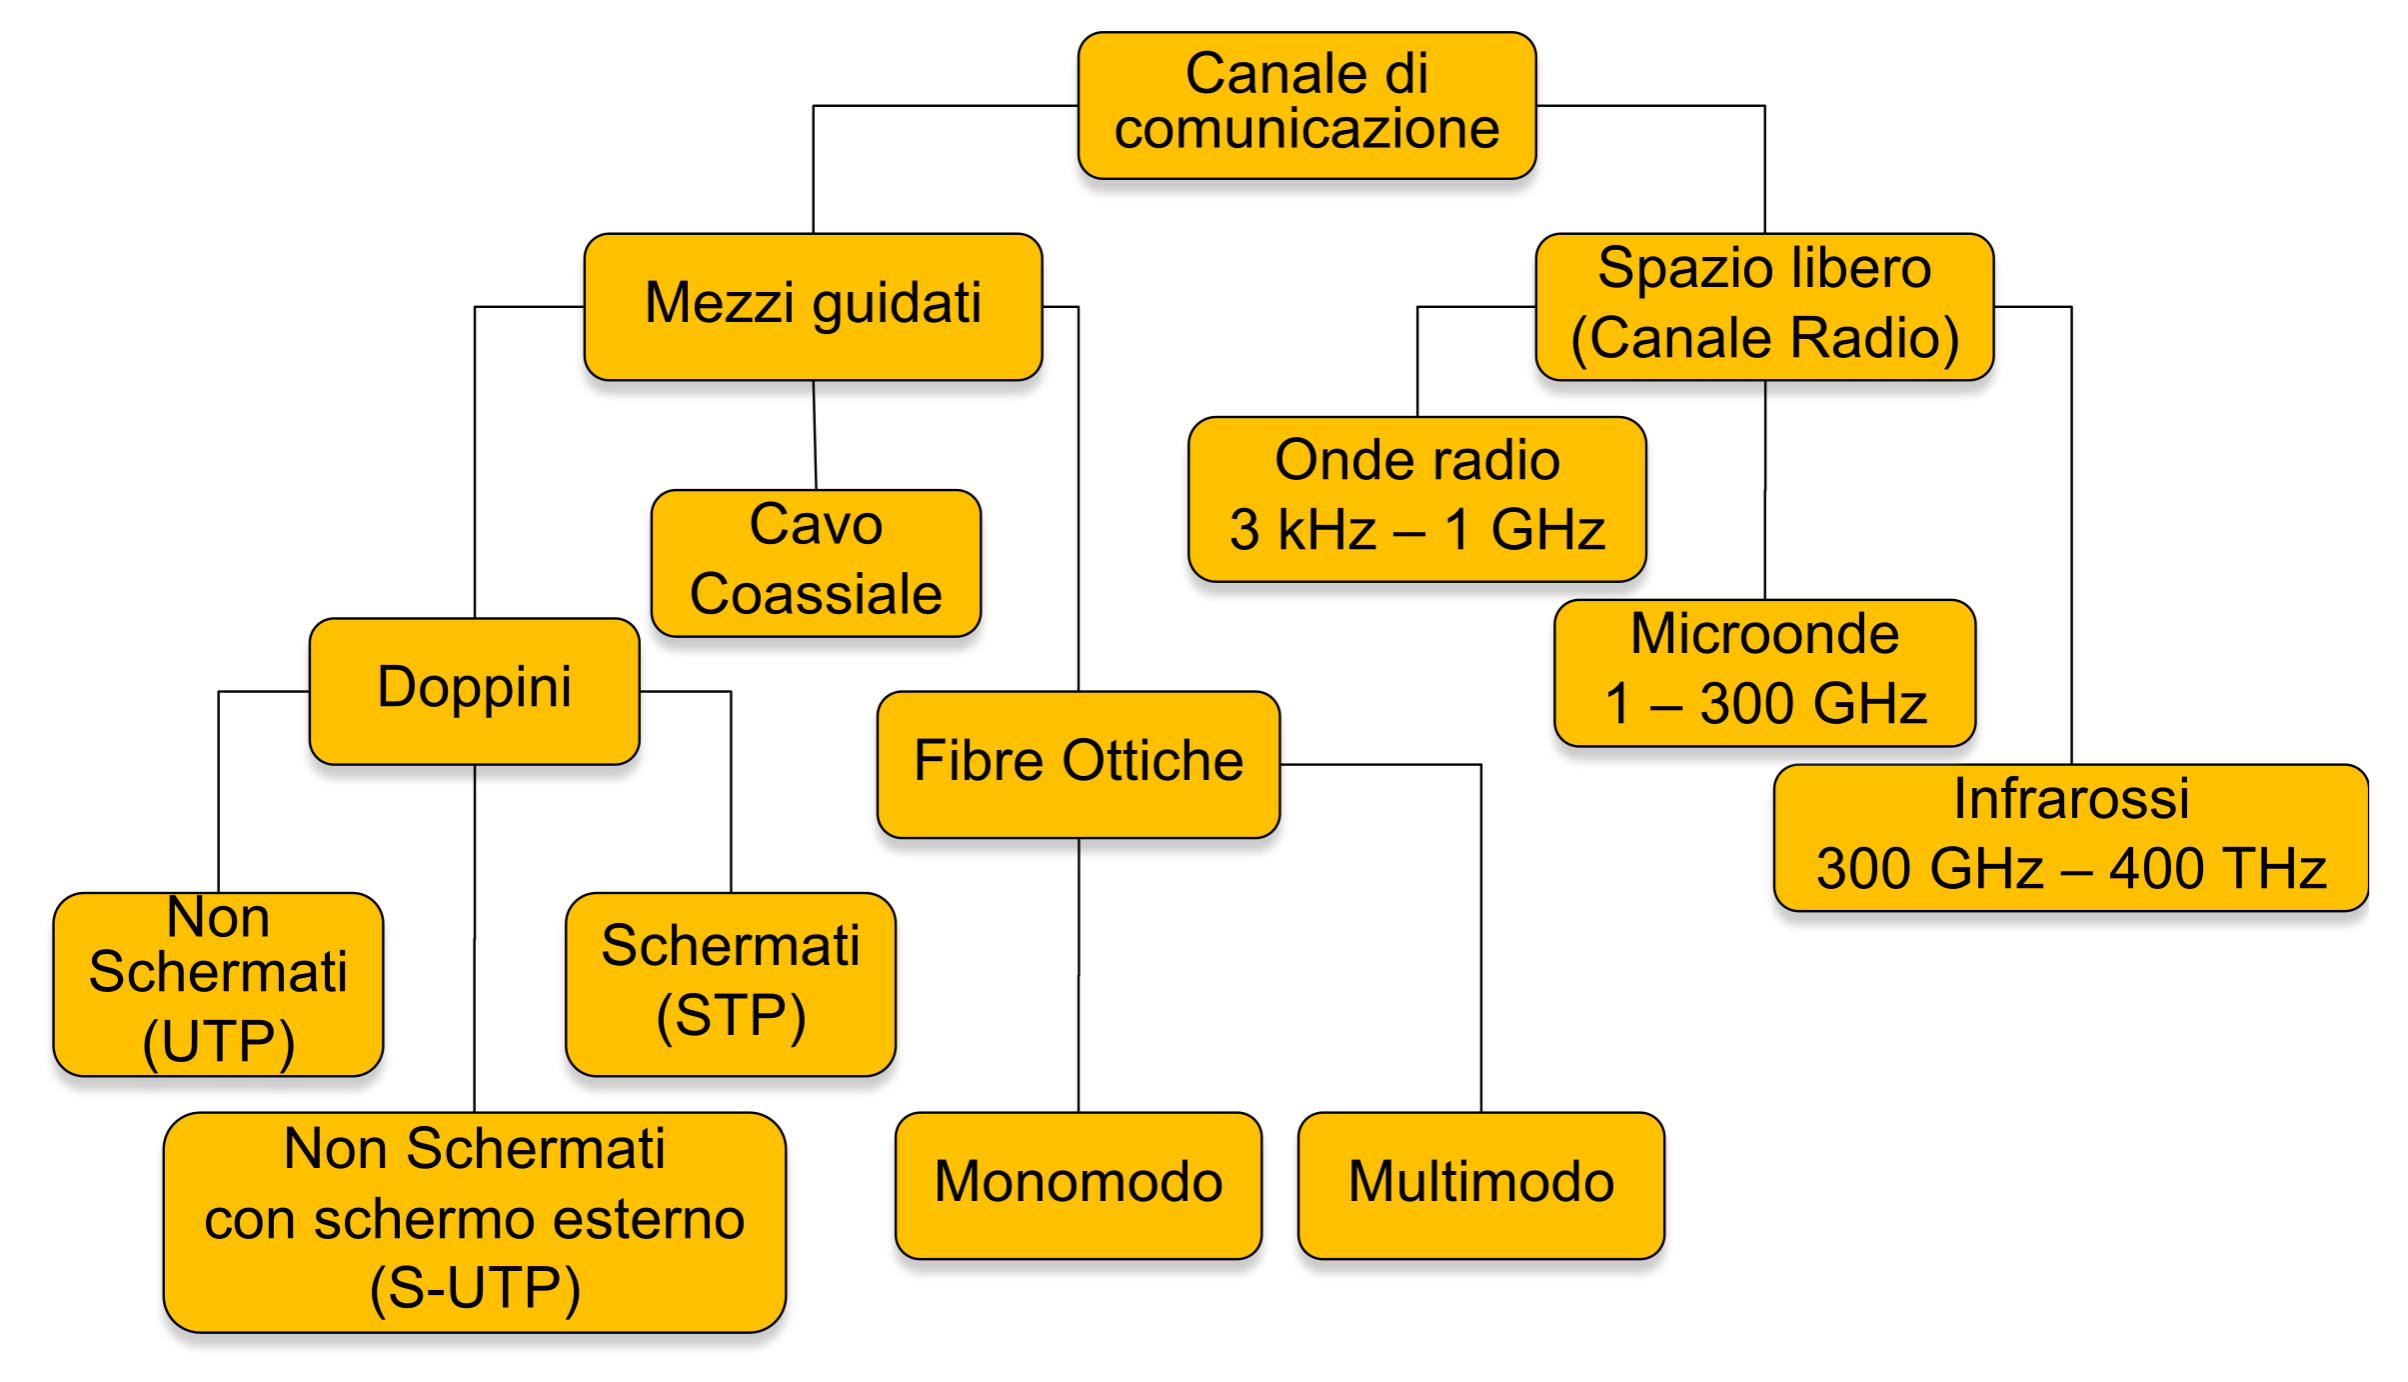
\includegraphics[width=1.05\textwidth]{images/canali_comunicazione}
    \caption{Tipi di canali di comunicazione}
    \label{fig:canali_comunicazione}
\end{figure}
\newpage
\section{Reti di telecomunicazioni - basi}
\subsection{Commutazione di circuito e commutazione di pacchetto}
\paragraph{Commutazione di circuito}
Si usava negli anni 20 del 900, quando chiamavo qualcuno inserivo il numero e nella centrale c’era qualcuno che fisicamente connetteva il mio cavo con quello a cui corrisponde il numero che ho digitato, rendendo il mezzo di comunicazione tra le due persone lo stesso cavo.
\paragraph{Commutazione di pacchetto} 
l'informazione viene impacchettata e divisa in unità, questo vuol dire che ci saranno dei ritardi dovuti a quest'impacchettamento. Le informazioni riguardanti il pacchetto stesso sono contenute nell'header, mentre nel payload c'è l'informazione, i dati che voglio trasportare. 
i nodi intermedi decidono come gestire il trasporto(commutazione) di tali pacchetti leggendo il contenuto dell’header. l’operatore ha un miglior uso di risorse.
un problema è che arrivano più pacchetti allo stesso nodo e devono attendere la commutazione del nodo che è arrivato prima.

\begin{figure}[h!]
    \centering
    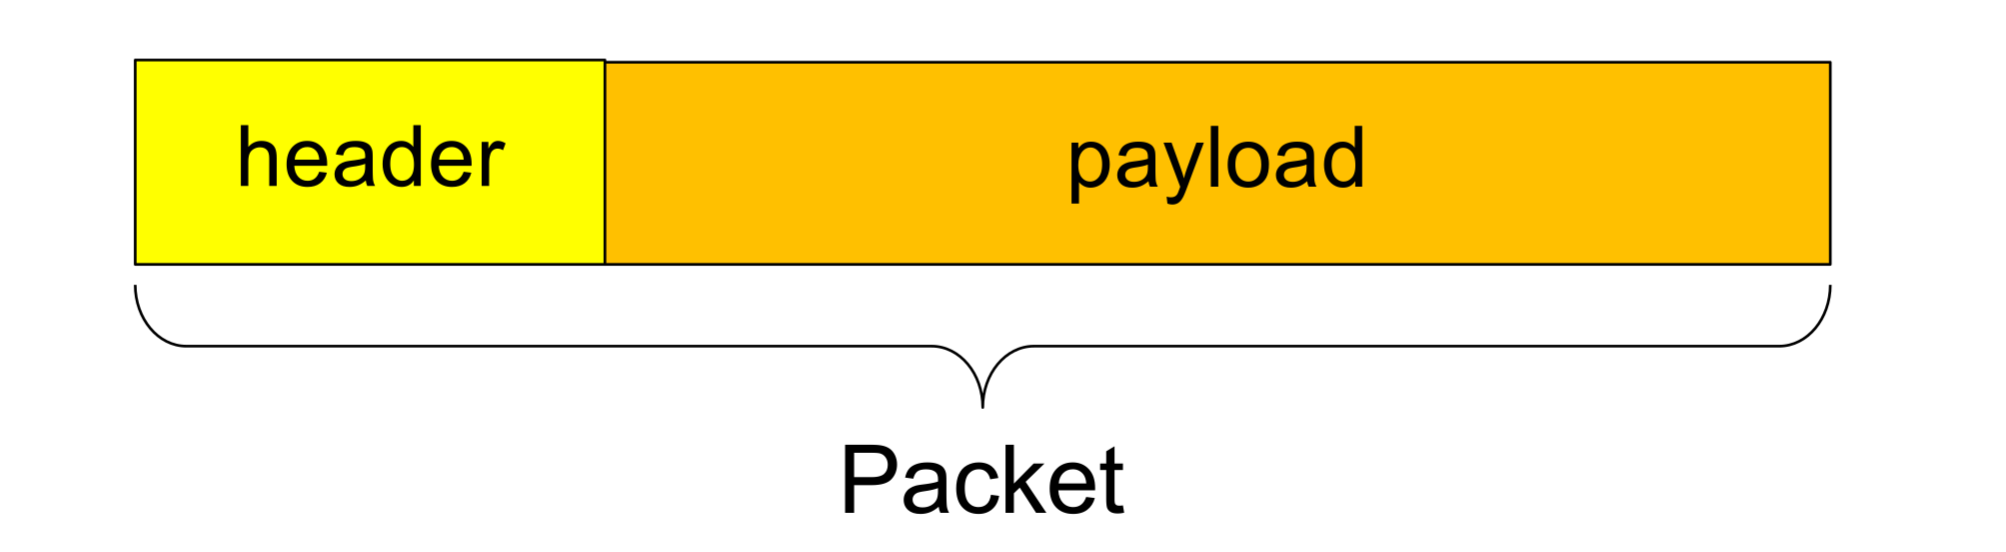
\includegraphics[width=1.05\textwidth]{images/pacchetto_generico.png}
    \caption{Commutazione di pacchetto}
    \label{fig:commutazione_pacchetto}
\end{figure}

Due tipi di commutazione di pacchetto: 
\begin{itemize}
    \item Datagram: ogni pacchetto, che prende il nome di datagramma, contiene nell’header le informazioni del mittente e destinatario. i nodi decidono la strada che deve fare il pacchetto(routing), questo viene fatto
    \item Virtual circuit: la comunicazione avviene in 3 fasi (setup, data
exchange, teardown) e l'instradamento è effettuato solo durante il setup.
Pertanto tutti i pacchetti vengono instradati lungo lo stesso percorso
(circuito), ma i nodi intermedi non devono ogni volta rieffettuare il routing,
ma solo lo switching (inoltrare il pacchetto dall'ingresso all'uscita corretta).
\end{itemize}
\newpage
\subsection{Ritardo end-to-end}
Il ritardo end-to-end è il tempo che intercorre tra l'invio di un pacchetto da parte del mittente e la ricezione dello stesso pacchetto da parte del destinatario. Questo ritardo è influenzato da diversi fattori, tra cui il tipo di rete, la distanza tra i nodi, la congestione della rete e le caratteristiche dei nodi stessi. 

Il ritardo nell'invio di un'informazione da mittente a destinatario ha più componenti:
    \begin{description}
        \item[Ritardo di trasmissione:] è il tempo necessario a inviare i bit sul mezzo, $T_f = \frac{L}{C}$, ad esempio il ritardo per la trasmissione di 1000 bit (informazione) su un cavo (canale) da 1 Gbit, $T_f = \frac{1000}{10^9}$, dove $L$ è la lunghezza in bit dell'informazione, $C$ è la frequenza di cifra.

        \item[Ritardo di propagazione:] è il tempo impiegato dai dati per attraversare la rete, tipicamente è il tempo che impiegano le onde elettromagnetiche a viaggiare in un mezzo di una certa lunghezza: $t = \frac{d}{v}$, dove $v$ è la velocità di propagazione (velocità della luce) e $d$ è la distanza considerata.

        \item[Ritardo di elaborazione:] $T_p$, è il tempo necessario all'elaborazione di un pacchetto in un nodo, dipende dalla velocità di calcolo dei processori.

        \item[Ritardo in accodamento:] $T_q$, tempo di attesa in coda nel buffer di ricezione e dipende dal traffico generato da tutti i flussi che attraversano il nodo in considerazione, è quello più difficile da prevedere e calcolare.
    \end{description}
    \begin{figure}[h!]
        \centering
        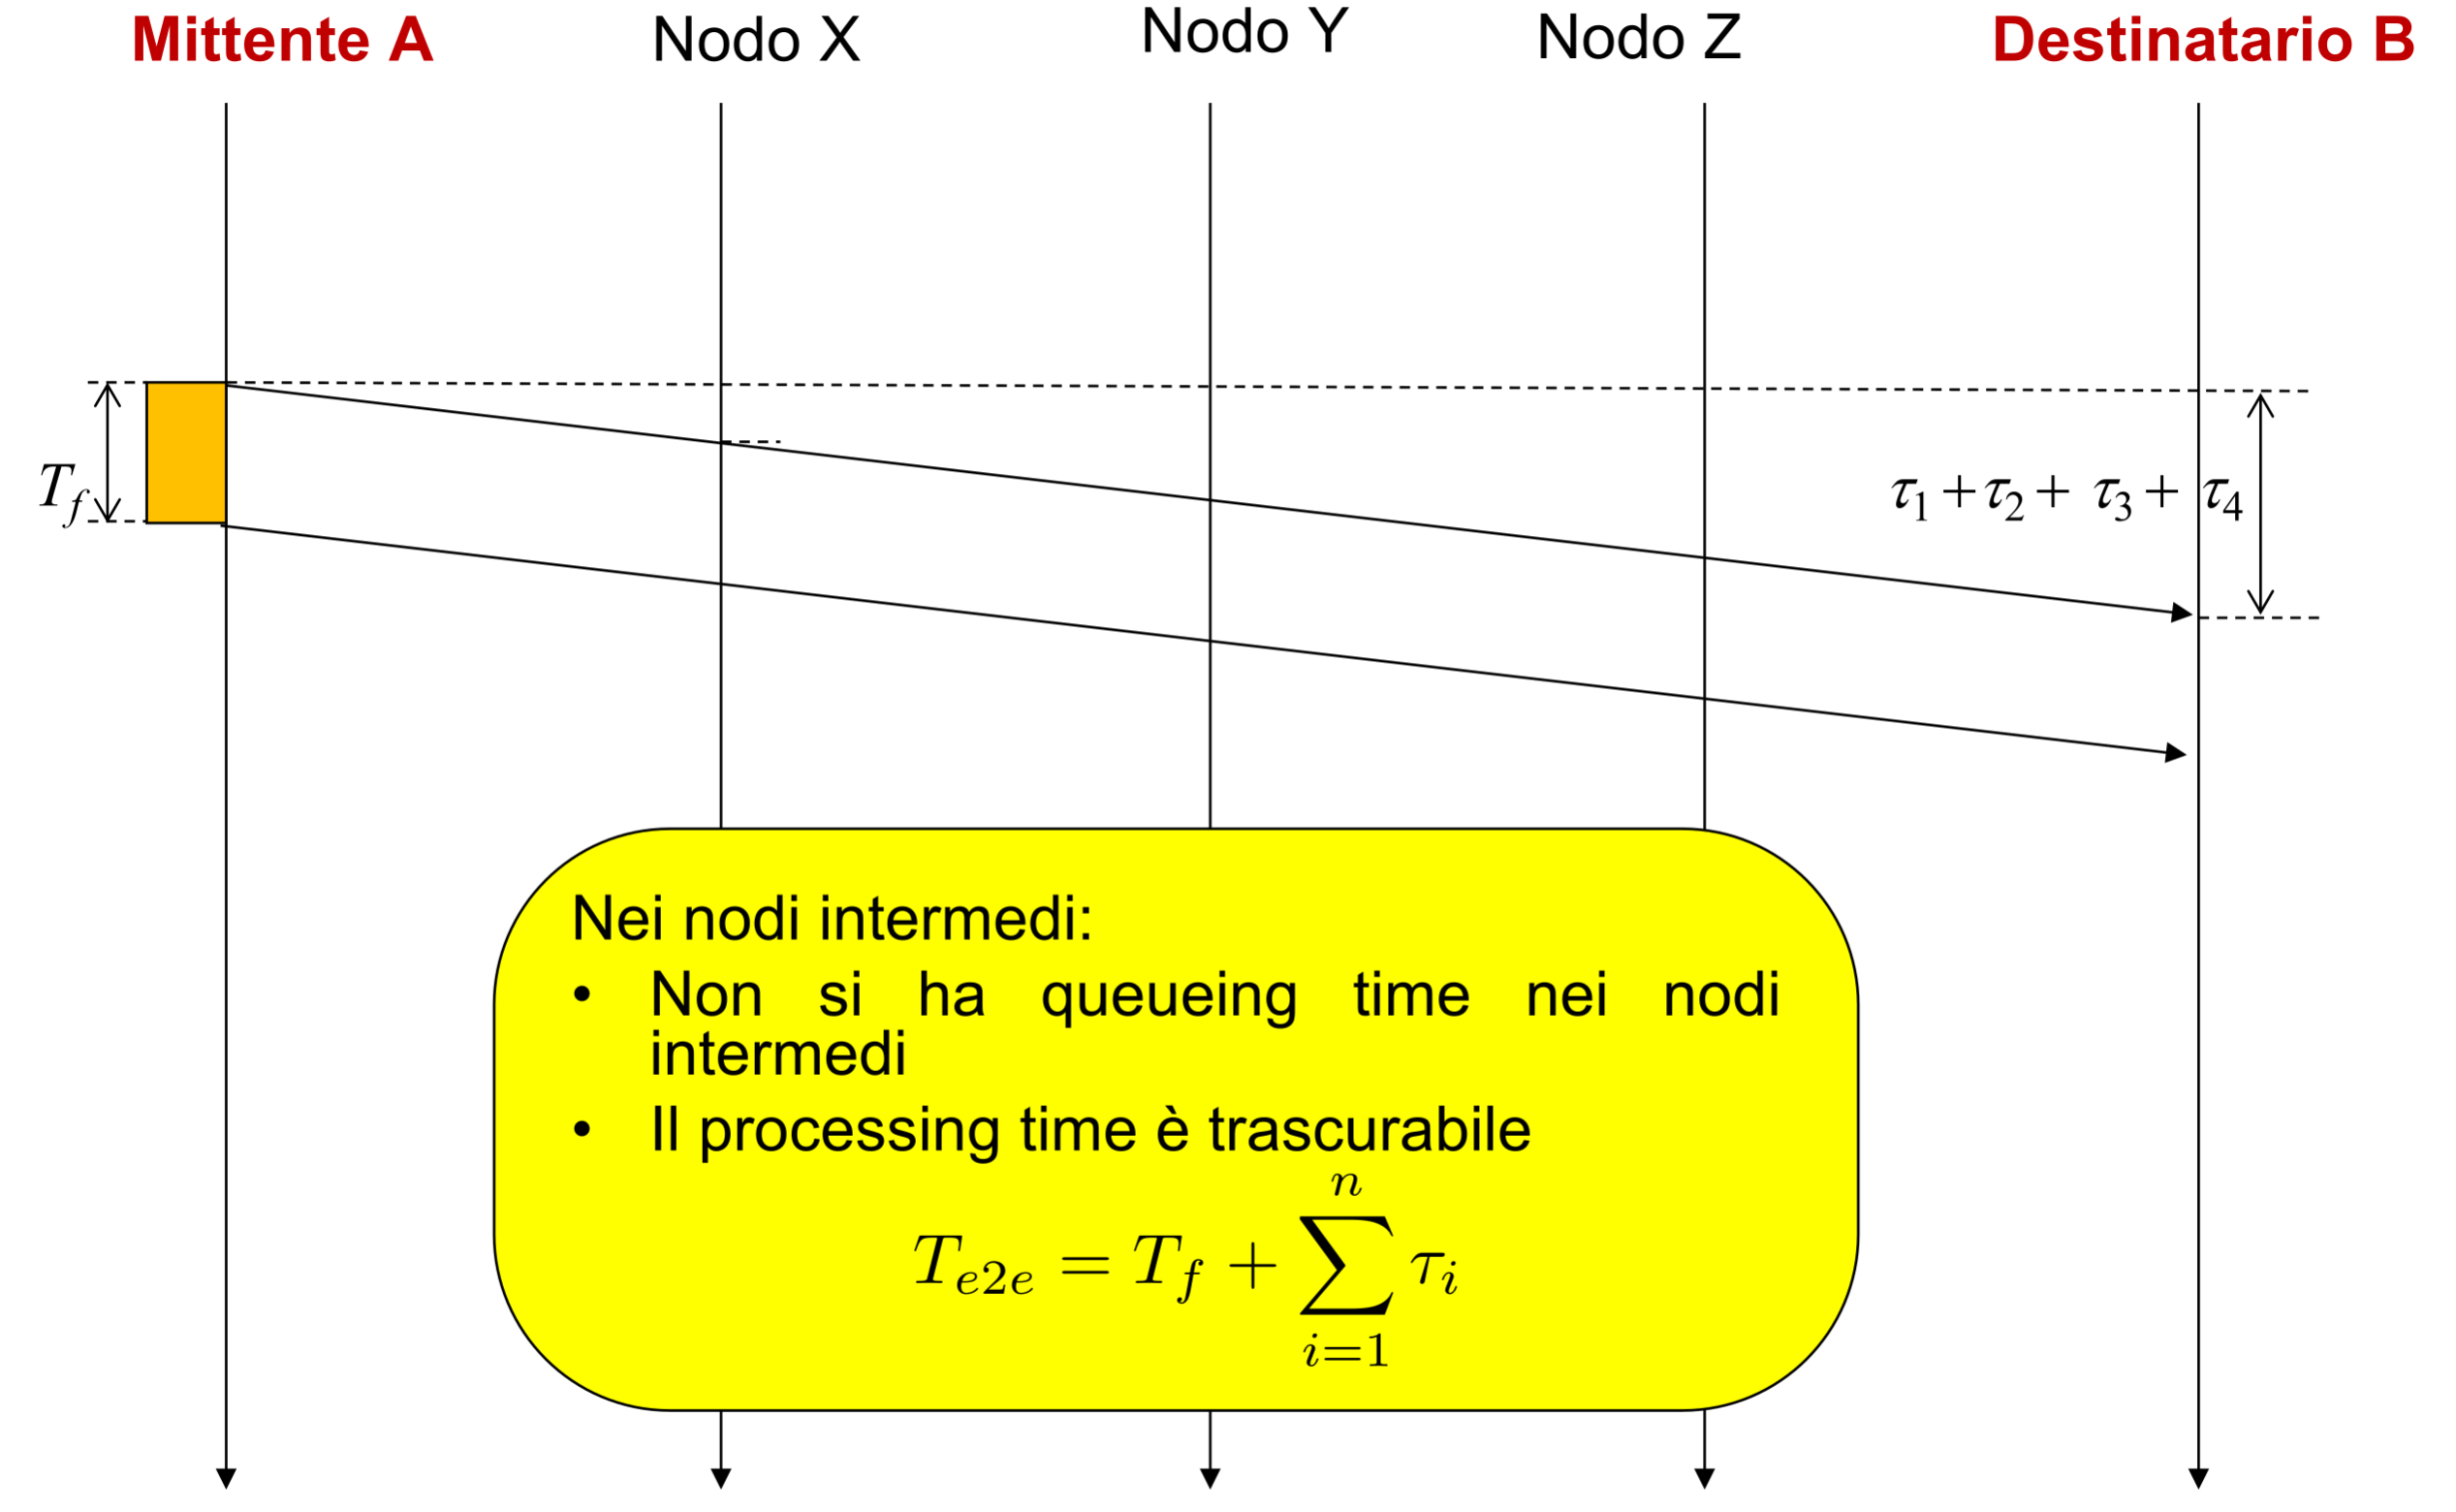
\includegraphics[width=1\textwidth]{images/e2e_circuit_switching.png}
        \caption{Ritardo e2e circuit switching: sommo i ritardi dovuti al mezzo(ritardo di trasmissione) e i ritardi dovuti alla propagazione nel mezzo}
        \label{fig:circuit_switching}
    \end{figure}
    
    
    \begin{figure}[h!]
        \centering
        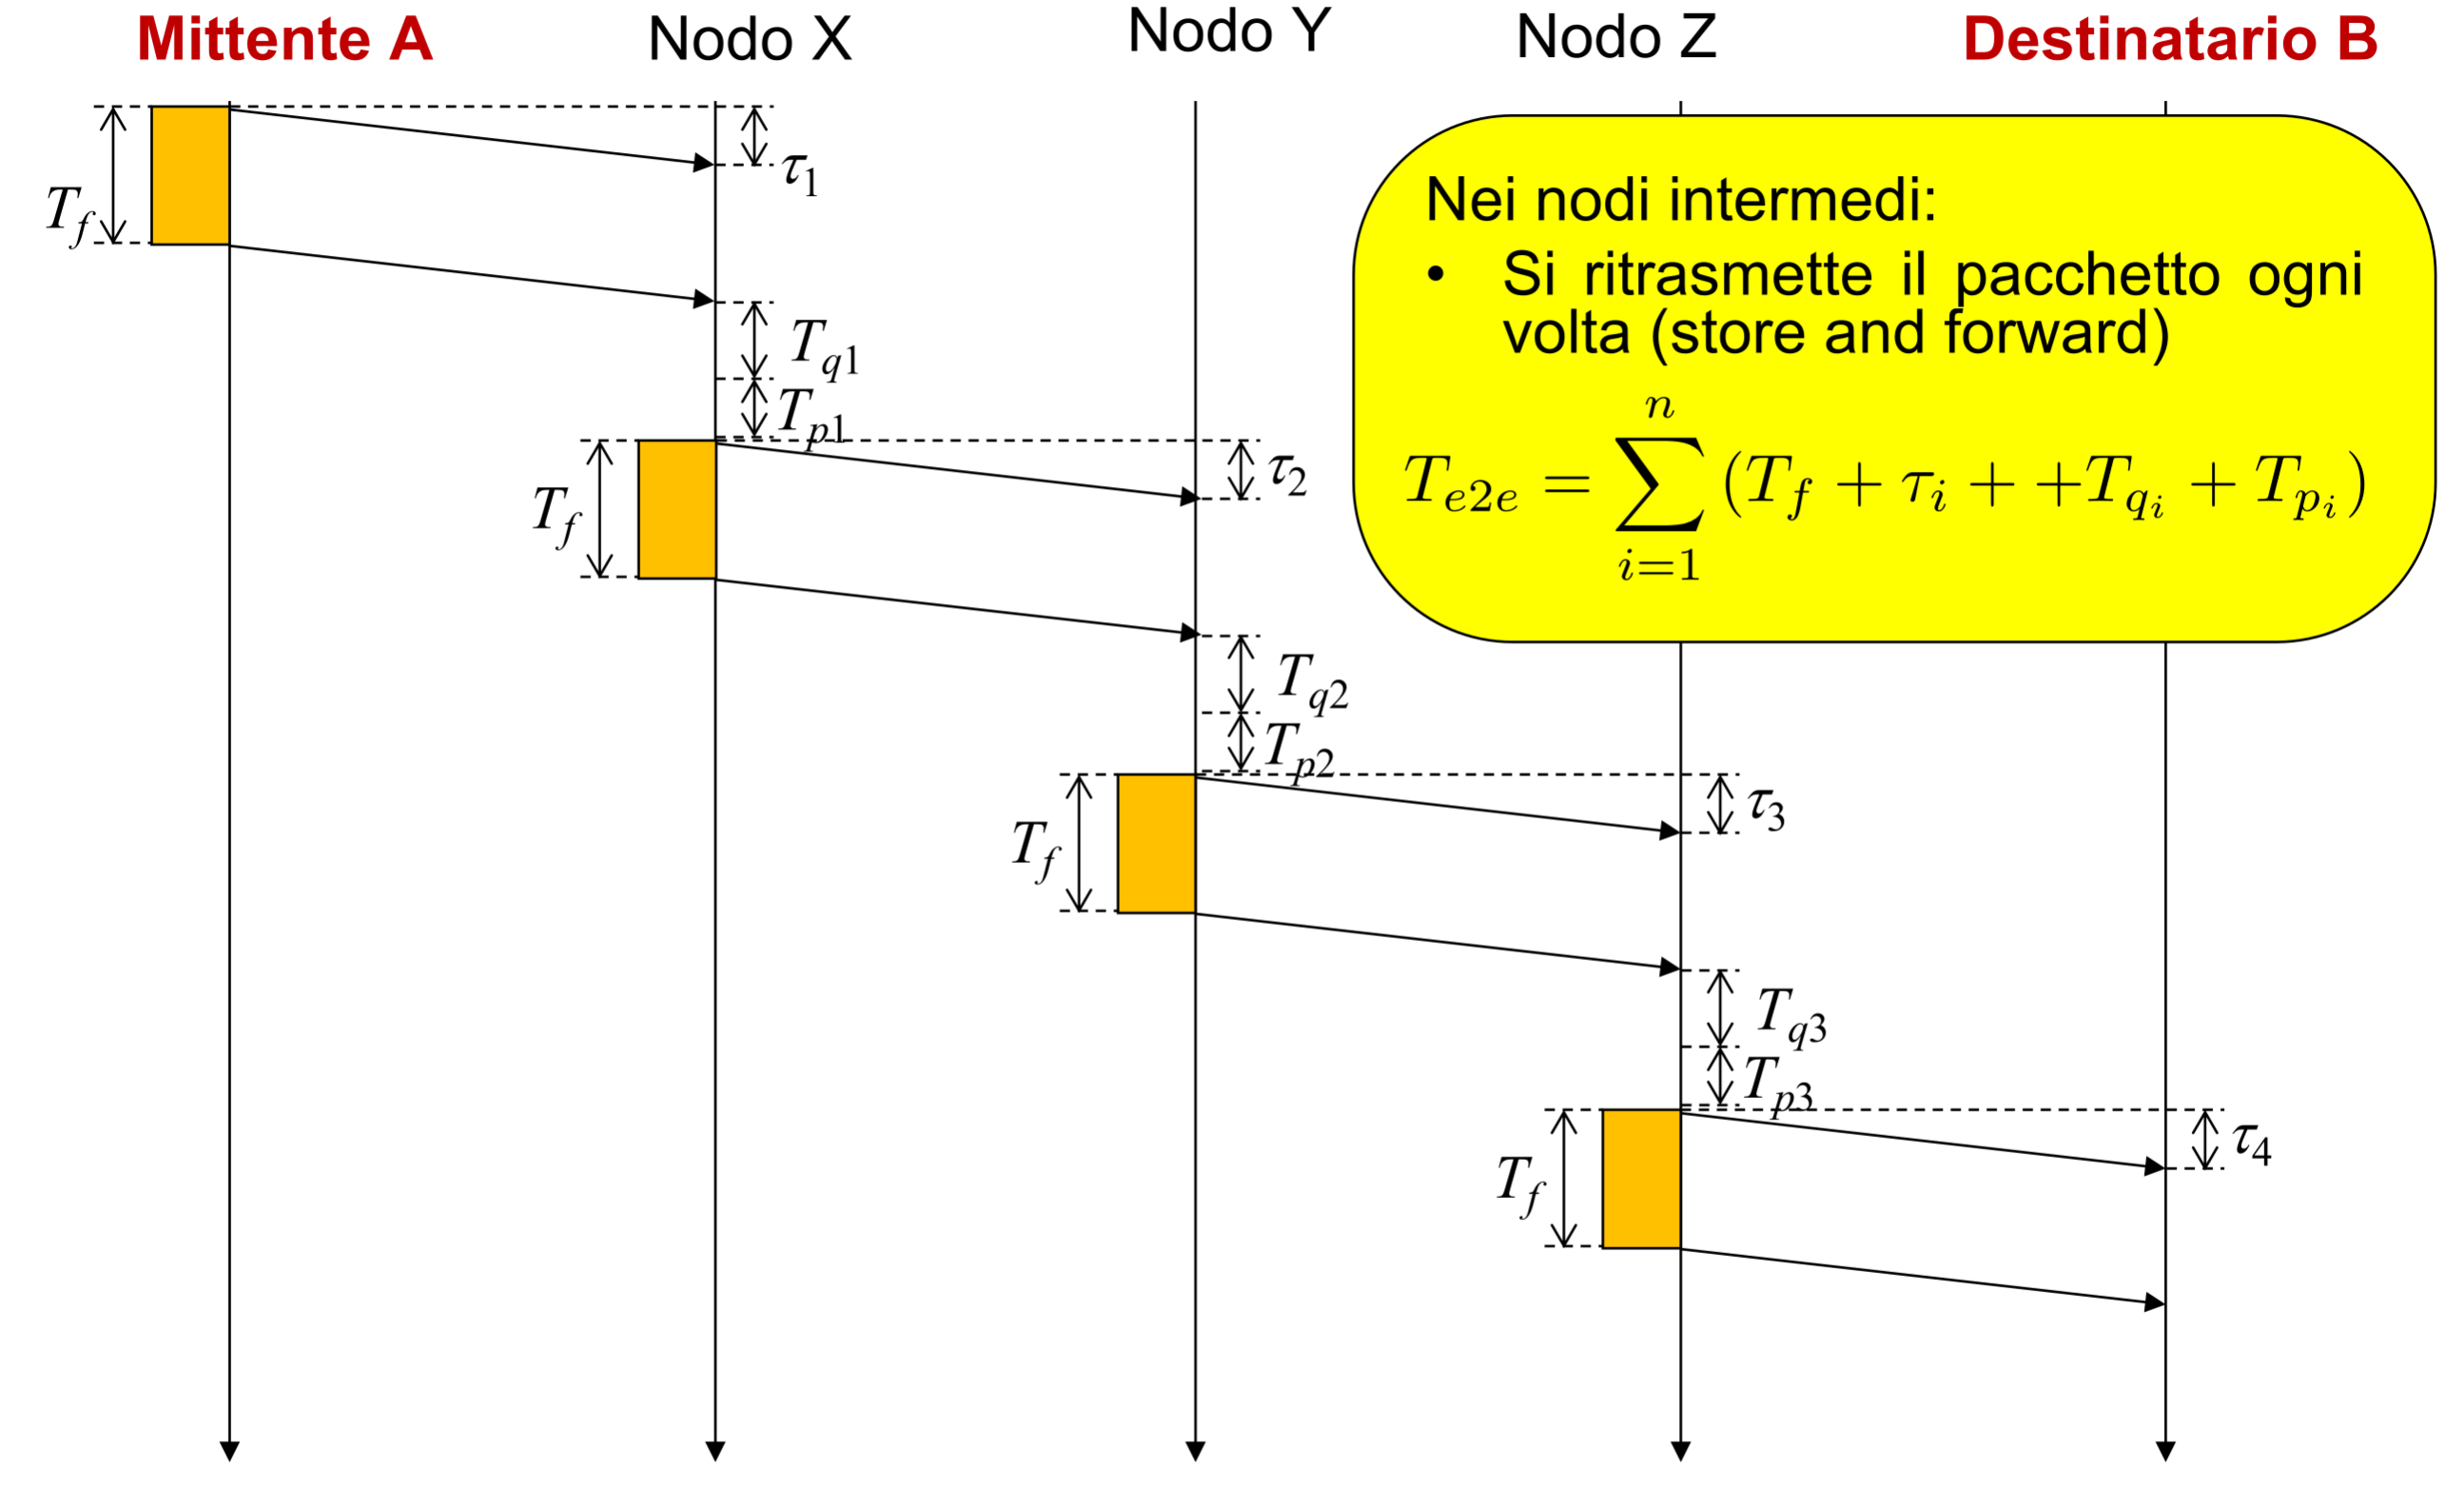
\includegraphics[width=1\textwidth]{images/e2e_packet_switching.png}
        \caption{Ritardo e2e packet switching: (sommo TUTTI i ritardi)
il packet switching ha una latenza maggiore rispetto al circuit switching}
        \label{fig:packet_switching}
    \end{figure}